\documentclass[a4paper,12pt]{article}
\usepackage{amsmath}
\usepackage{url}
\usepackage{amssymb}
\usepackage{graphicx}
%\documentclass{article}
\usepackage{setspace, enumitem,titlesec}
\usepackage{calc}
			% Activate to display a given date or no date
\usepackage{mathtools}
\usepackage{mathrsfs }
\DeclarePairedDelimiter\ceil{\lceil}{\rceil}
\DeclarePairedDelimiter\floor{\lfloor}{\rfloor}
\usepackage{algorithm}
\usepackage{algorithmic}
\usepackage{fancybox}
%################
\usepackage{float}
\usepackage{makecell}
\usepackage{bbm}
\usepackage{amsmath}
\usepackage{amssymb}
\usepackage{amsthm}
\usepackage{cite}
\usepackage{authblk}
%\usepackage{algpseudocode}

%\renewcommand{\thepseudonum}{\roman{pseudonum}}
\renewcommand\labelenumi{(\theenumi)}
%vector
\renewcommand{\vec}[1]{\mathbf{#1}}
\title {A study of the spherical coordinates parameterization}
%\author{jim.morris.shen@gmail.com}
%\author{The Graduate Center, City University of New York}
\author{Xiaoke Shen}
\affil{the Graduate Center, the City University of New York}
\date{}
\begin{document}
\maketitle

\begin{abstract}
This report provides the results of using the spherical coordinates to resolve the constrained problems.
\end{abstract}
%\textbf{Due Mar 1st 11:59 pm. 10 points for each exercise and 20 points for the extra credit exercise }\\
\section{Introduction}
For the resource allocation problem, suppose resource $p_i$ is allocated to $i$ where $i$ is the index of the object which get the resource, $p_i$ is the allocation ratio to the total available resource. Then we can get:\\
\begin{equation} \label{eq:sum_res_alo}
\sum_{i=1}^{n} p_i = 1
\end{equation}

We can rewrite the equation \ref{eq:sum_res_alo} as bellow:\\
\begin{equation} \label{eq:sum_res_alo_r_2}
\sum_{i=1}^{n} (r_i)^2 = 1
\end{equation}
Any feasible allocation vector $r = (r_1,...,r_n)$ on the unit ball can be described through $n-1$ angels denoted by $\theta_i, 1\leq i \leq n-1$, in the following way. Indeed, the spherical coordinated parameterization of $r$ via $\theta^T = (\theta_1,...,\theta_{n-1}) $ is given by:\\



\begin{equation}\label{eq:sphe}
    r_i(\theta)=\left\{
                \begin{array}{ll}
                  cos(\theta_1), \quad \quad \quad \quad \quad \quad \quad \quad i=1;\\
                  cos(\theta_i)\prod_{k=1}^{i-1} sin(\theta_k),\quad  \quad  2\leq i \leq n-1;\\
                  sin(\theta_{n-1})\prod_{k=1}^{n-2} sin(\theta_k),\quad  i=n.
                \end{array}
              \right.
\end{equation}

\subsection{Penalty Methods}
In order to adress the constrained optimization problem, several methods are provided. In this work, the penalty method is studied to compare the performance of the spherical coordinated parameterization method.\\
Given the constrained problem as described in equation \ref{eq:pena_1}
\begin{equation}\label{eq:pena_1}
\begin{aligned}
\min_{x\in \mathbb{R}^n}J(x), \\
\textrm{s.t.} \quad & 0 \leq x_i \leq 1, i=1,...,n\\
              \quad & \sum_{i=1}^{n} x_i = 1\\
\end{aligned}
\end{equation}
THe penalty methods modify the original performance function to penalize the extent to which the constraints are not satisfied. Recall that $|.|$ denotes the Euclidean norm, then the penalized function is defined:\\
\begin{equation} \label{eq:pena_2}
\begin{aligned}
J_{\alpha}(x) = J(x)+\frac{\alpha}{2}(|g(x)_{+}|^2+|g(x)_{\_}|^2),\\
where \quad g(x)_{+} =(g_1(x)_{+},...g_j(x)_{+})^T, and \quad g_i(x)_{+} = max(1,g_i(\theta))-1\\
where \quad g(x)_{\_} =(g_1(x)_{\_},...g_j(x)_{\_})^T, and \quad g_i(x)_{\_} = min(0,g_i(\theta))\\
\end{aligned}
\end{equation}
Then two-time scale algorithm is used to get the optimal value of $x$ by using the formulas shown in equation \ref{eq:pena_a}, equation \ref{eq:pena_b} and equation \ref{eq:pena_c}. \\
\begin{equation} \label{eq:pena_a}
x_{n+1}=x_n-\epsilon _n \nabla J{\alpha_ n}(x_n)^T
\end{equation}
\begin{equation}\label{eq:pena_b}
\alpha_{n+1}=\alpha_n+\delta _n \mathbbm{1} _{\{n\in {T_i}\}}
\end{equation}
where $\sum \delta_n = + \infty$, and\\
\begin{equation}\label{eq:pena_c}
\nabla J{\alpha_ n}(x_n) =\nabla _x J(x_n)+\alpha_n(g(x_n)^T \nabla g(x_n) \mathbbm{1}_{\{|g(x_n)|<0\}}+g(x_n)^T \nabla g(x_n) \mathbbm{1}_{\{|g(x_n)|>1\}})
\end{equation}
%\begin{table*}[!ht]
%\begin{center}
%\begin{tabular}{|c|c|c|}
%\hline
%No. & $X_i$ and $n$ of $X_i$&Satisfy requirement of which Theorem\\
%\hline
%1 & \makecell{$X_i \sim \mathcal{N}(0,1)$ \\$n \sim \mathcal{U}\{1,100\} $}& %Theorem 1\\
%\hline
%2 & \makecell{$X_i \sim \mathcal{U}(-1,1)$ or\\ $\mathcal{U}(-10,10)$  with equal chance \\$n \sim \mathcal{U}\{1,100\} $}& Theorem 2\\
%\hline
%\end{tabular}
%\end{center}
%\caption{Experiments for Theorem 1 and Theorem 2. The $\mathcal{U}\{1,100\}$ means  discrete uniform distribution}
%\label{tab:expe12}
%\end{table*}


\section{Deterministic Optimization}
\subsection{Cost function is linear function}
\subsubsection{Plots of the cost function }
In this experiment, the cost function is a linear function. The optimization problem is described as below:\\


\begin{equation}\label{eq:1}
\begin{aligned}
\min_{x_1,x_2\in \mathbb{R}} \quad & J(x_1,x_2) = -2x_1-x_2\\
\textrm{s.t.} \quad & 0 \leq x_1 \leq 1\\
              \quad & 0 \leq x_2 \leq 1\\
              \quad & \sum_{i=1}^{2} x_i = 1\\
\end{aligned}
\end{equation}


As $\sum_{i=1}^{2} x_i = 1$, we can change equation \ref{eq:1} to:\\
\begin{equation}\label{eq:2}
\begin{aligned}
\min_{x\in \mathbb{R}} \quad & J(x) = -x-1\\
\textrm{s.t.} \quad & 0 \leq x \leq 1\\
\end{aligned}
\end{equation}






\begin{figure}[H]
\begin{center}
%\fbox{\rule{0pt}{2in} \rule{.9\linewidth}{0pt}}
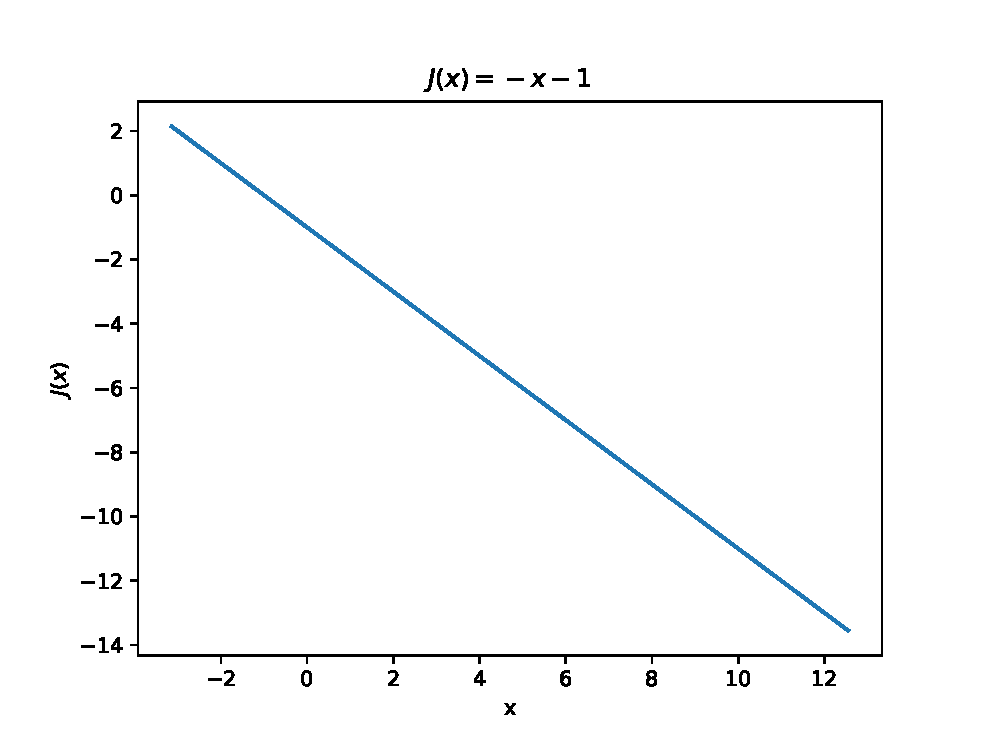
\includegraphics[width=1.0\linewidth]{line.eps}

\end{center}
   \caption{The plot of the cost function: $J(x) = -x-1$.  }
\label{fig:line_cost}
\end{figure}

\begin{equation}\label{eq:line_theta}
\begin{aligned}
\min_{\theta\in \mathbb{R}} \quad & J(\theta) = -cos(\theta)^2-1\\
\end{aligned}
\end{equation}

The plot of the equation \ref{eq:2} is shown in figure \ref{fig:line_cost}. By using the equation \ref{eq:sphe}, we can change the constrained optimization problem to an unconstrained problem by using the spherical coordinates parameterization method. The unconstrained problem by using the spherical coordinates parameterization method is formally described in equation \ref{eq:line_theta}. The plot of the equation \ref{eq:line_theta} is shown in figure \ref{fig:line_cost_sphe}.\\  


%\begin{equation}
%\begin{aligned}
%\min_{w,b,\xi} \quad & \frac{1}{2}w^{t}w+C\sum_{i=1}^{N}{\xi_{i}}\\
%\textrm{s.t.} \quad & y_{i}(w\phi(x_{i}+b))+\xi_{i}-1\\
%  &\xi\geq0    \\
%\end{aligned}
%\end{equation}



\begin{figure}[H]
\begin{center}
%\fbox{\rule{0pt}{2in} \rule{.9\linewidth}{0pt}}
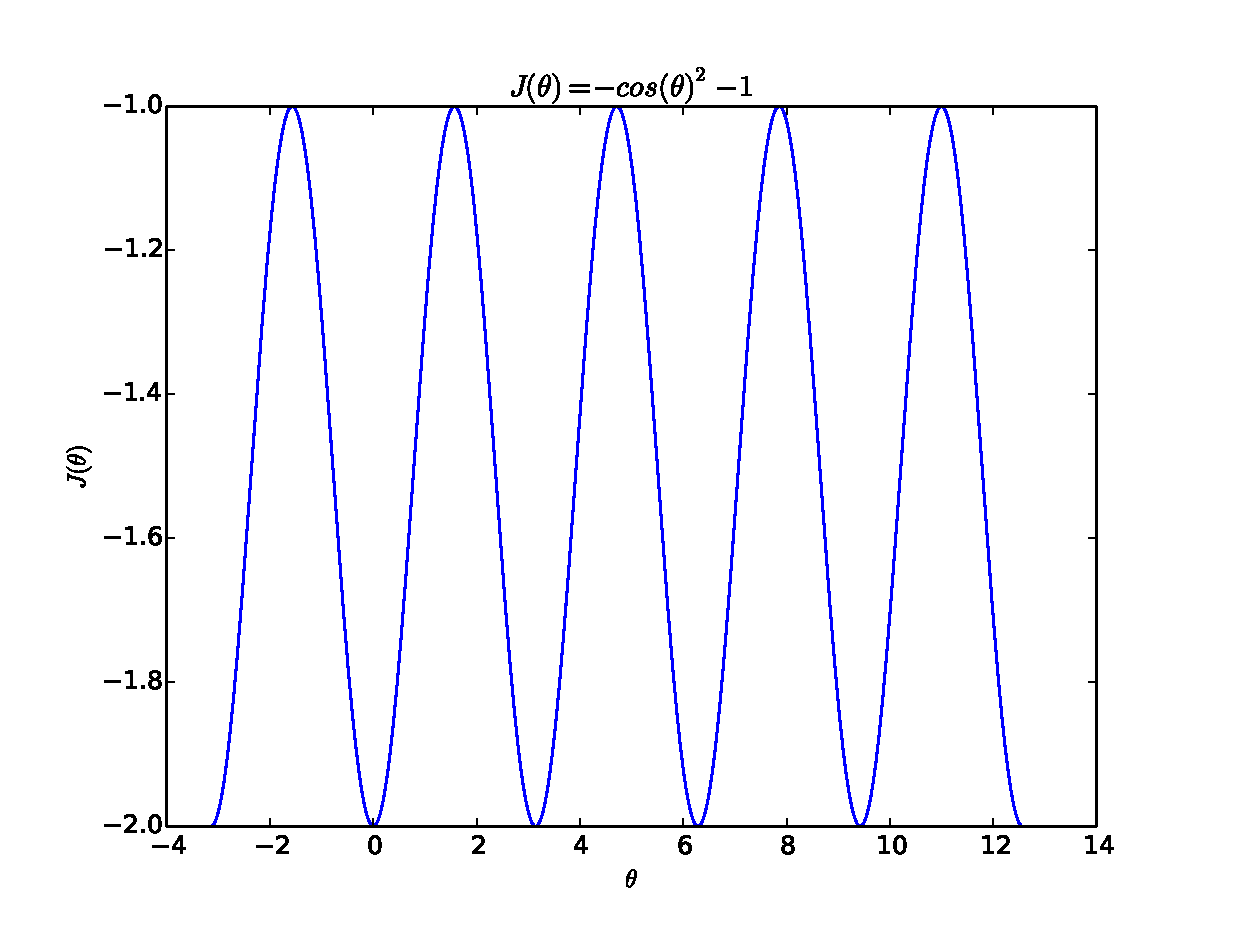
\includegraphics[width=1.0\linewidth]{line_sphe.eps}


\end{center}
   \caption{The plot of the cost function: $J(\theta) = -cos(\theta)^2-1$. }
\label{fig:line_cost_sphe}
\end{figure}


\subsubsection{Penalty method }
 By using the equation \ref{eq:pena_a}, equation \ref{eq:pena_b} and equation \ref{eq:pena_c}, for this specified question, we can get:\\
\begin{equation} \label{eq:pena_line_a}
x_{n+1}=x_n-\epsilon _n \nabla J{\alpha_ n}(x_n)^T
\end{equation}
\begin{equation}\label{eq:pena_line_b}
\alpha_{n+1}=\alpha_n+\delta _n \mathbbm{1} _{\{n\in {T_i}\}}
\end{equation}

\begin{equation}\label{eq:pena_line_c}
\nabla _x J(x_n) = -1
\end{equation}

\begin{equation}\label{eq:pena_line_d}
\nabla J{\alpha_ n}(x_n) =\nabla _x J(x_n)+\alpha_n x_n( \mathbbm{1}_{\{x_n<0\}}+ x_n \mathbbm{1}_{\{x_n>1\}})
\end{equation}

By using the equation \ref{eq:pena_line_a} , equation \ref{eq:pena_line_b},  equation \ref{eq:pena_line_c}  and equation \ref{eq:pena_line_d}, we can estimate the optimal value of $x$ and the estimation process is shown in figure \ref{fig:line_result}\\

\begin{figure}[H]
\begin{center}
%\fbox{\rule{0pt}{2in} \rule{.9\linewidth}{0pt}}
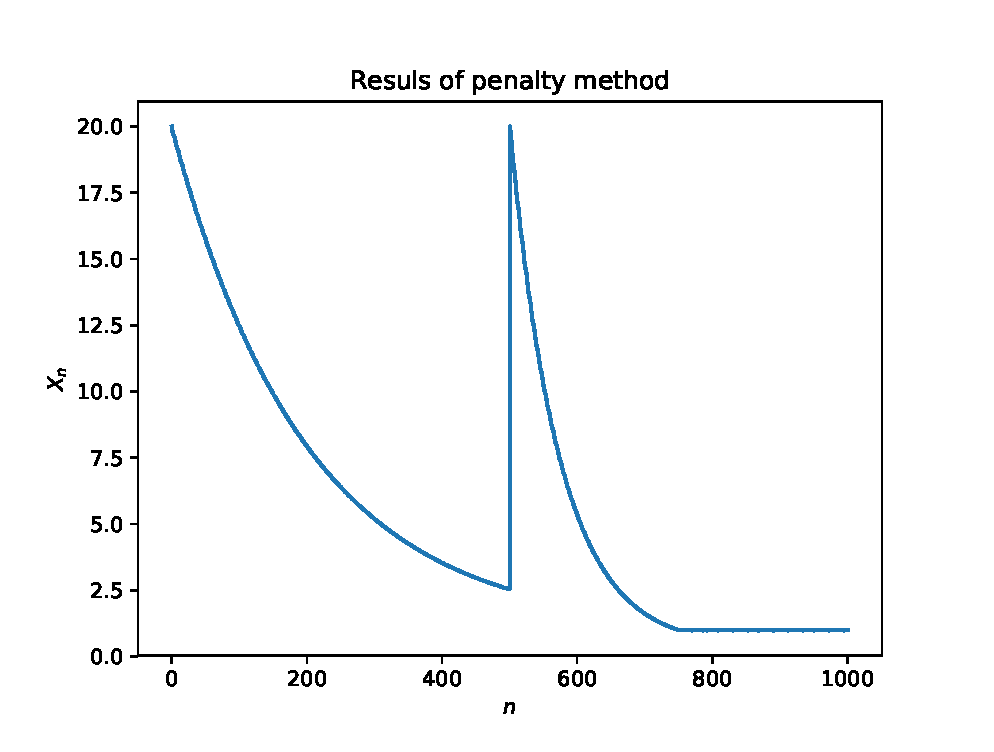
\includegraphics[width=1.0\linewidth]{line_est.eps}


\end{center}
   \caption{The estimation process of the optimal $x$ when the penalty method is used.Here the initial value of $x$ is set to 20. The total iteration for $T_i$ is 500. The $\alpha_1 = 1$ and $\alpha _{n+1} = \alpha _n + \delta_n,$ where $\delta _ n=e^n$. }
\label{fig:line_result}
\end{figure}


\subsubsection{the spherical coordinated parameterization method }

\begin{equation} \label{eq:sphe_line_a}
\theta_{n+1}=\theta_n-\epsilon _n \nabla J{\theta_ n}
\end{equation}
\begin{equation}\label{eq:sphe_line_b}
\nabla _{\theta} J(\theta_n) = 2*cos(\theta_n)*sin(\theta_n)
\end{equation}

When the spherical coordinated parameterization is used, the constrained optimization problem can be changed into a unconstrained problem. We can use the formula shown in equation \ref{eq:sphe_line_a} and equation \ref{eq:sphe_line_b} to estimate the optimal result. As we don't know whether the cost function is convex, we may get multiple local minimum. In order to get a global minimum, several experiments are done to get more than one estimation and the best one will be selected as the global optimization. In this experiment, 5 experiments are done. The estimation process is  shown in figure \ref{fig:line_result_sphe}.\\
\begin{figure}[H]
\begin{center}
%\fbox{\rule{0pt}{2in} \rule{.9\linewidth}{0pt}}
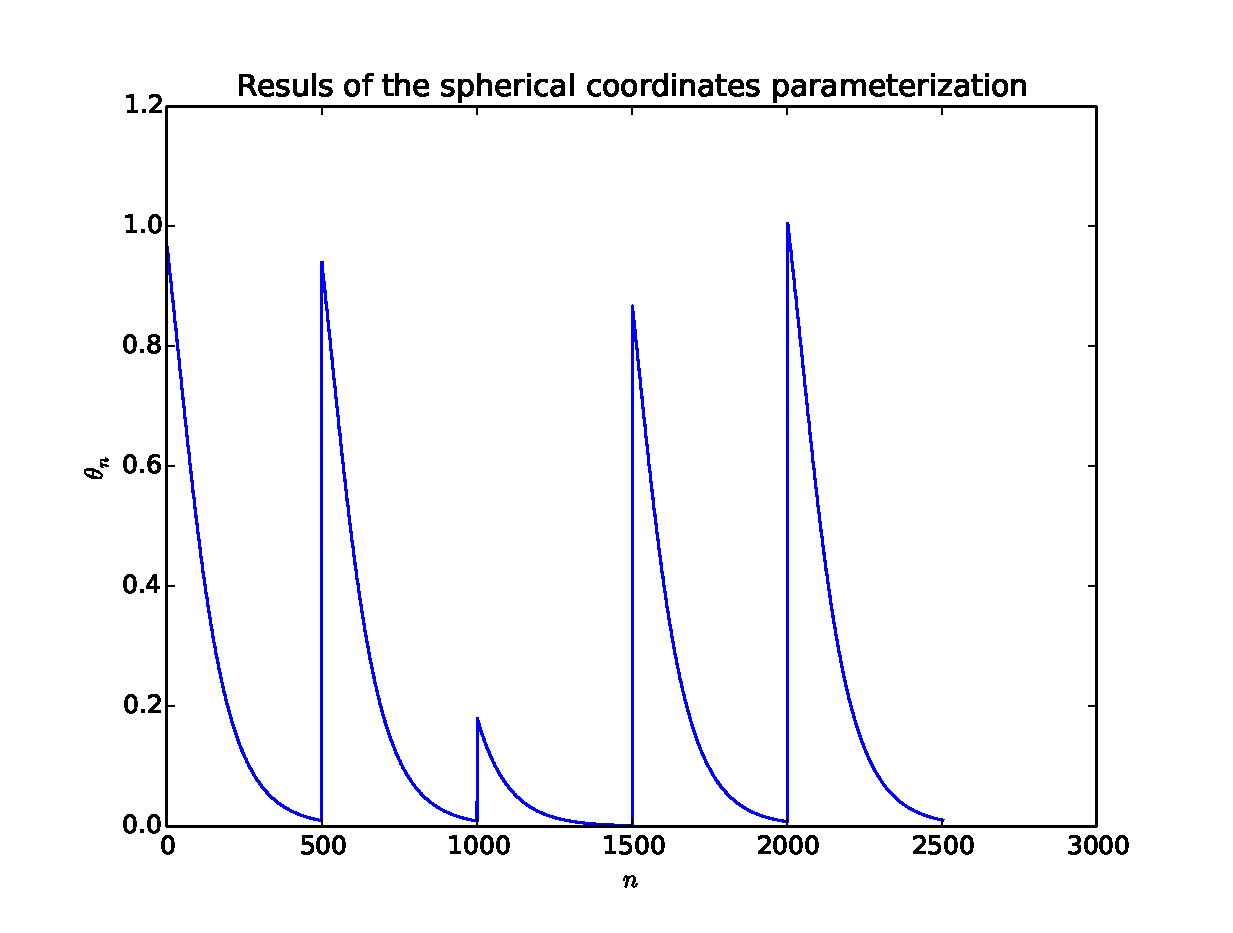
\includegraphics[width=1.0\linewidth]{line_est_sphe.eps}


\end{center}
   \caption{The estimation process of the optimal $\theta$ when the spherical coordinated parameterization is used. In order to make sure the global optimal value is collected, 5 times experiments with random initialized value of $\theta$ is done and the global minimum value is collected from those 5 experiments.}
\label{fig:line_result_sphe}
\end{figure}

\subsubsection{Optimization results comparison}



%owners-MacBook-Pro:project jimmy$ python line.py 
%i,a 0 1.0
%i,a 1 2.71828182846
%res 0.987424834706 0.994721377501
%--- 0.000710010528564 seconds ---
%owners-MacBook-Pro:project jimmy$ python line_sphe.py 
%i,a 0 0.620390355449
%i,a 1 0.598575782266
%i,a 2 0.114661879355
%i,a 3 0.552088529417
%i,a 4 0.63994160765
%res 0.999998638966
%--- 0.00955319404602 seconds ---


\begin{table*}[!ht]
\begin{center}
\begin{tabular}{|c|c|c|c|}
\hline
Optimal $x$& method & estimated $x$&execution time(ms)\\
\hline
1.0& penalty method&0.995&0.71\\
\hline
1.0&  \makecell{ the spherical coordinates \\parameterization}&1.000&9.55\\
%1.036 & 522.653 & 322.425& 17.956&$\mu = 522.653, \sigma =17.956$ &$\lambda =522.653 $\\
%1.645 & 194.570 & 168.123& 12.966&$\mu = 194.570, \sigma =12.966$ &$\lambda =194.570 $\\
%2.000 & 91.139 & 86.115& 9.280&$\mu = 91.139, \sigma =9.280$ &$\lambda =91.139 $\\
%2.800 & 10.440 & 10.228& 3.198&$\mu = 10.440, \sigma =3.198$ &$\lambda =10.440 $\\

\hline
\end{tabular}
\end{center}
\caption{The results of the penalty method and spherical coordinate parameterization.}
\label{tab:line}
\end{table*}

The comparison of the penalty and the spherical coordinates parameterization method is shown in table \ref{tab:line}. From the results, we can see that the  spherical coordinates parameterization method  can get a more accurate result. At the same time, the spherical coordinates parameterization method is slower as 5 repeated experiments are done to get the global minimum result. \\

%\begin{table*}[!ht]
%\begin{center}
%\begin{tabular}{|c|c|c|c|c|c|}
%\hline
%thre. $u$&mean &variance&std & Gaussian Parameters&Poisson Parameters \\
%\hline

%1.036 & 522.653 & 322.425& 17.956&$\mu = 522.653, \sigma =17.956$ &$\lambda =522.653 $\\
%1.645 & 194.570 & 168.123& 12.966&$\mu = 194.570, \sigma =12.966$ &$\lambda =194.570 $\\
%2.000 & 91.139 & 86.115& 9.280&$\mu = 91.139, \sigma =9.280$ &$\lambda =91.139 $\\
%2.800 & 10.440 & 10.228& 3.198&$\mu = 10.440, \sigma =3.198$ &$\lambda =10.440 $\\

%\hline
%\end{tabular}
%\end{center}
%\caption{Statistic results and empirical disturibution parameters of $\mathbf{K}$ when the threshold $m=4096$}
%\label{tab:k}
%\end{table*}

\subsection{Cost function is polynomial }
\subsubsection{Plots of the cost function }
In this experiment, the cost function is a linear function. The optimization problem is described as below:\\
\begin{equation}\label{eq:pol2}
\begin{aligned}
\min_{x\in \mathbb{R}} \quad &J(x) =-x^4+2x^2-x\\
\textrm{s.t.} \quad & 0 \leq x \leq 1\\
\end{aligned}
\end{equation}
By using this cost function, we can get a minimum value which is between 0 and 1. We can change the problem as below by using the spherical coordinates parameterization method.\\




\begin{equation}\label{eq:poly_theta}
\begin{aligned}
\min_{\theta\in \mathbb{R}} \quad &J(\theta) = -cos(\theta)^8+2cos(\theta)^4-cos(\theta)^2\\
\end{aligned}
\end{equation}

The plot of the equation \ref{eq:pol2} is shown in figure \ref{fig:poly_cost}.  The plot of the equation \ref{eq:line_theta} is shown in figure \ref{fig:poly_cost_sphe}.\\  


\begin{figure}[H]
\begin{center}
%\fbox{\rule{0pt}{2in} \rule{.9\linewidth}{0pt}}
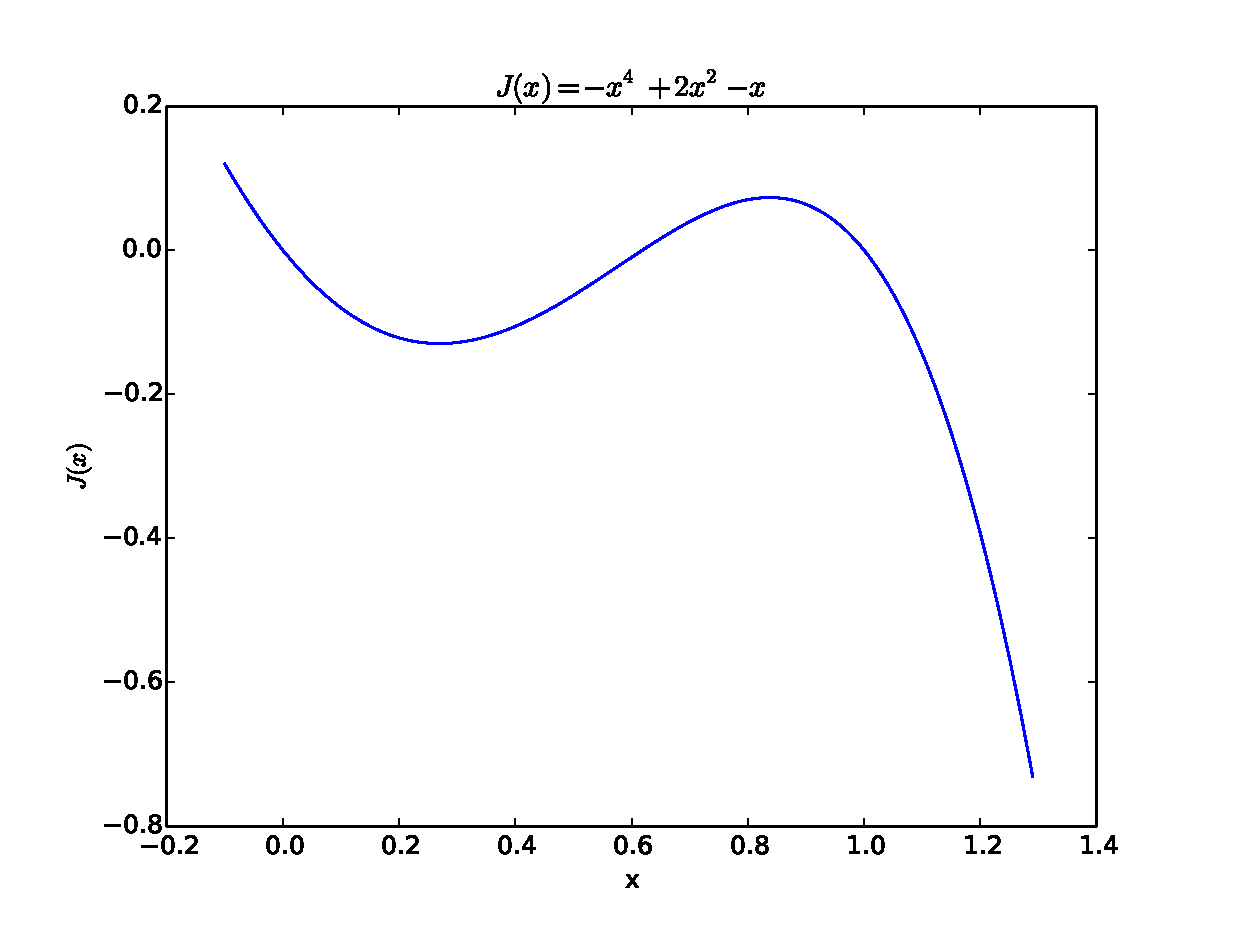
\includegraphics[width=1.0\linewidth]{polynomial.eps}


\end{center}
   \caption{The plot of the cost function: $J(x) =-x^4+2x^2-x$. }
\label{fig:poly_cost}
\end{figure}



\begin{figure}[H]
\begin{center}
%\fbox{\rule{0pt}{2in} \rule{.9\linewidth}{0pt}}
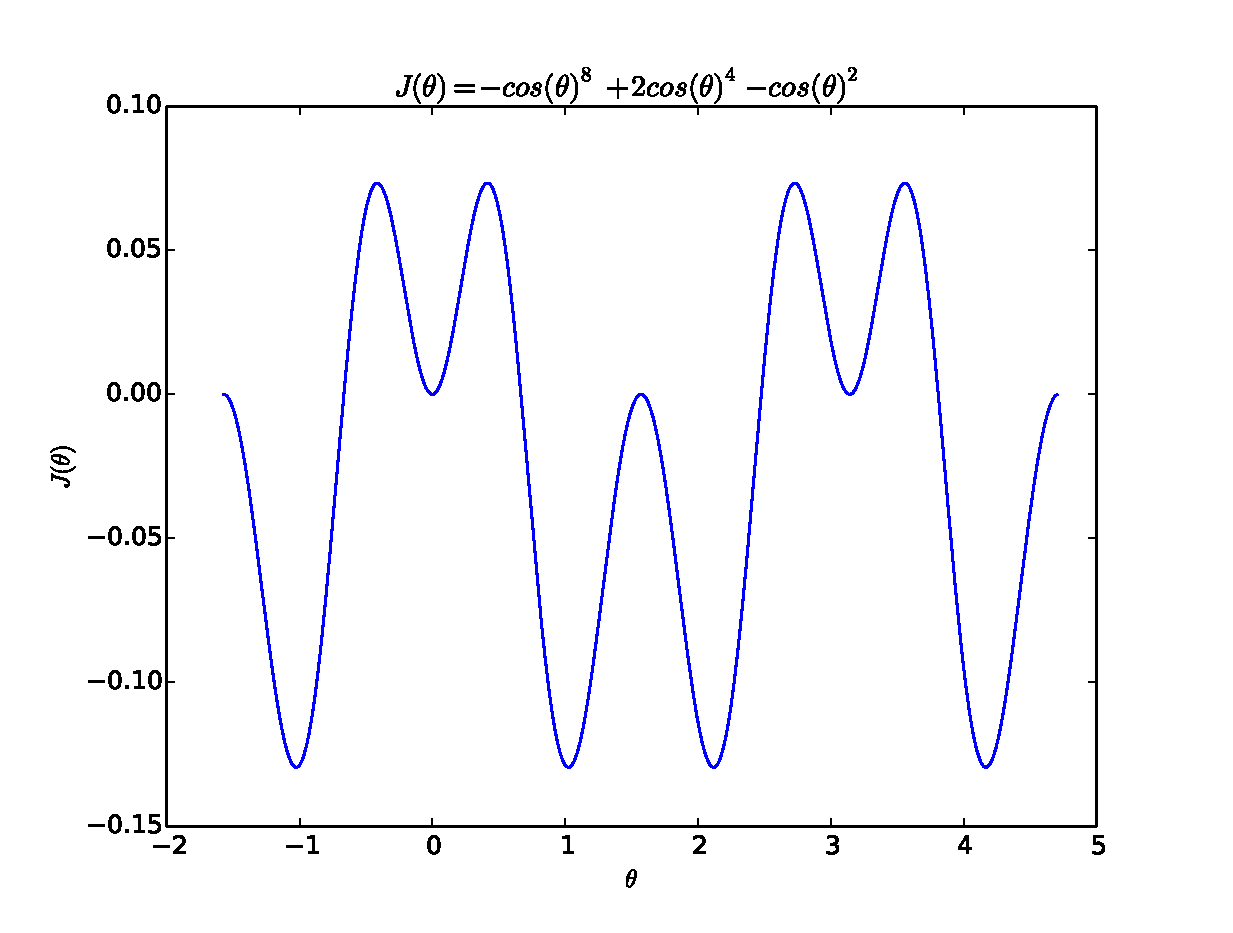
\includegraphics[width=1.0\linewidth]{polynomial_sphe.eps}


\end{center}
   \caption{The plot of the cost function: $J(\theta) = -cos(\theta)^8+2cos(\theta)^4-cos(\theta)^2$. }
\label{fig:poly_cost_sphe}
\end{figure}




\subsubsection{Penalty method }
 By using the equation \ref{eq:pena_a}, equation \ref{eq:pena_b} and equation \ref{eq:pena_c}, for this specified question, we can get:\\
\begin{equation} \label{eq:pena_poly_a}
x_{n+1}=x_n-\epsilon _n \nabla J{\alpha_ n}(x_n)^T
\end{equation}
\begin{equation}\label{eq:pena_poly_b}
\alpha_{n+1}=\alpha_n+\delta _n \mathbbm{1} _{\{n\in {T_i}\}}
\end{equation}

\begin{equation}\label{eq:pena_poly_c}
\nabla _x J(x_n) = -4x^3+4x-1
\end{equation}

\begin{equation}\label{eq:pena_poly_d}
\nabla J{\alpha_ n}(x_n) =\nabla _x J(x_n)+\alpha_n x_n( \mathbbm{1}_{\{x_n<0\}}+ x_n \mathbbm{1}_{\{x_n>1\}})
\end{equation}

By using the equation \ref{eq:pena_poly_a} , equation \ref{eq:pena_poly_b},  equation \ref{eq:pena_poly_c}  and equation \ref{eq:pena_poly_d}, we can estimate the optimal value of $x$ and the estimation process is shown in figure \ref{fig:poly_result}\\

\begin{figure}[H]
\begin{center}
%\fbox{\rule{0pt}{2in} \rule{.9\linewidth}{0pt}}
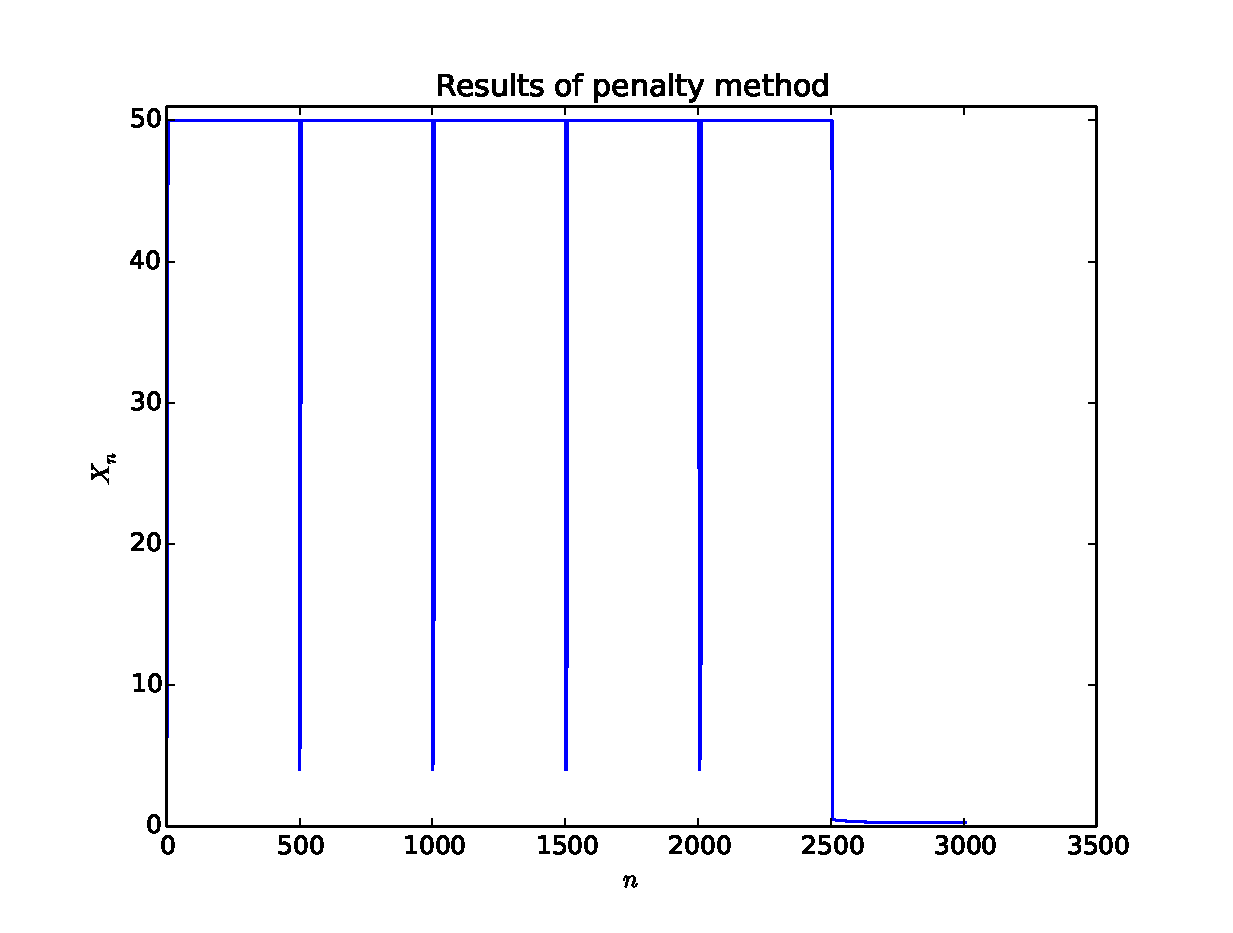
\includegraphics[width=1.0\linewidth]{polynomial_est.eps}


\end{center}
   \caption{The estimation process of the optimal $x$ when the penalty method is used.Here the initial value of $x$ is set to 4. The total iteration for $T_i$ is 500. The $\alpha_1 = 1$ and $\alpha _{n+1} = \alpha _n + \delta_n,$ where $\delta _ n=e^n$ The value of $x_n$ is upper bounded by the value of 50 as if it is not bounded, the value of $x_n$ will become too large to be handled by the computer. }
\label{fig:poly_result}
\end{figure}





\subsubsection{the spherical coordinated parameterization method }

\begin{equation} \label{eq:sphe_poly_a}
\theta_{n+1}=\theta_n-\epsilon _n \nabla J{\theta_ n}
\end{equation}
\begin{equation}\label{eq:sphe_poly_b}
\nabla _{\theta} J(\theta_n) = 8*cos(\theta_n)^7*sin(\theta_n)-8*cos(\theta_n)^3*sin(\theta_n)+2*cos(\theta_n)*sin(\theta_n)
\end{equation}

When the spherical coordinated parameterization is used, the constrained optimization problem can be changed into a unconstrained problem. We can use the formula shown in equation \ref{eq:sphe_poly_a} and equation \ref{eq:sphe_poly_b} to estimate the optimal result. As we don't know whether the cost function is convex, we may get multiple local minimum. In order to get a global minimum, several experiments are done to get more than one estimation and the best one will be selected as the global optimization. In this experiment, 5 experiments are done. The estimation process is  shown in figure \ref{fig:polynomial_est_res_sphe}.\\



\begin{figure}[H]
\begin{center}
%\fbox{\rule{0pt}{2in} \rule{.9\linewidth}{0pt}}
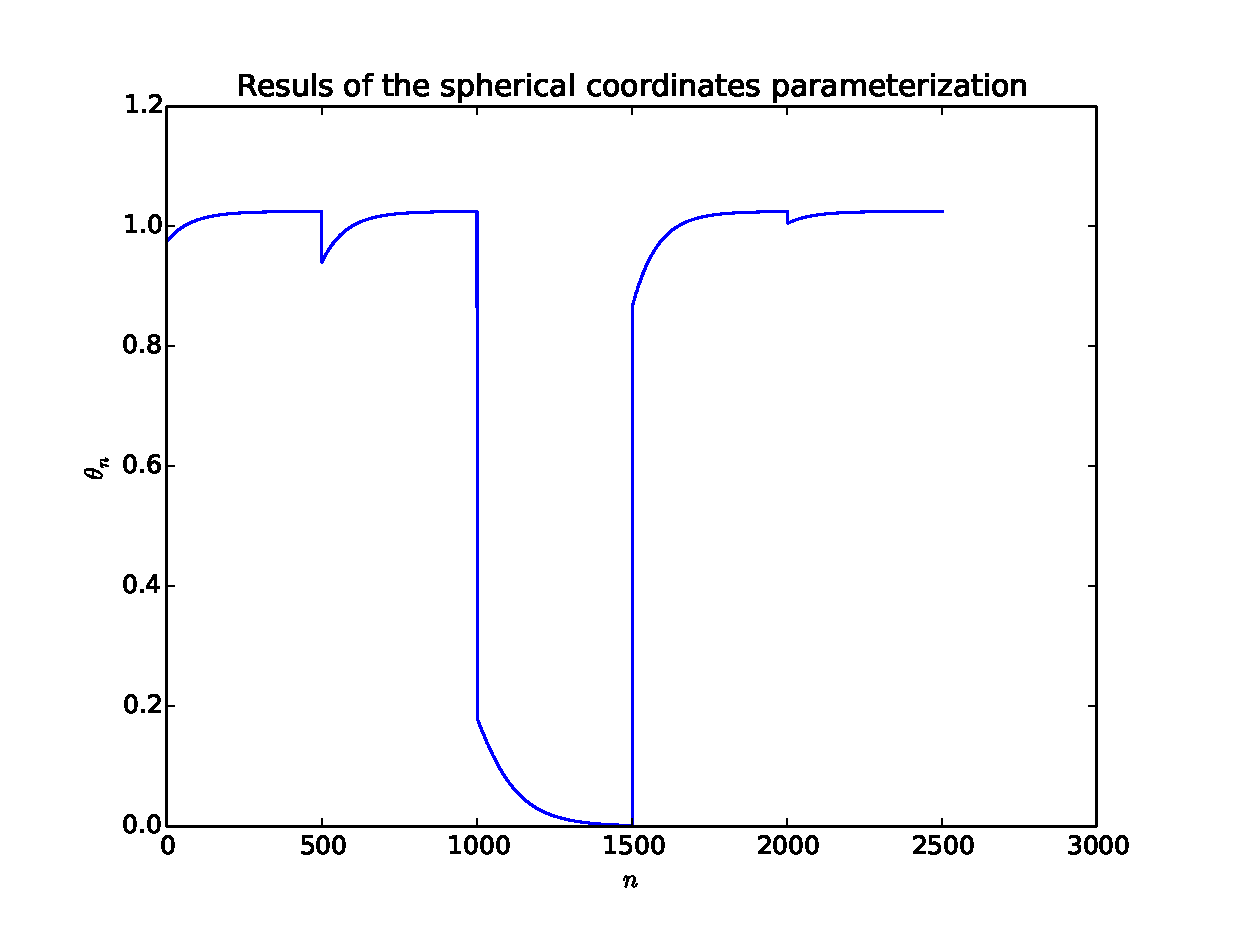
\includegraphics[width=1.0\linewidth]{polynomial_est_sphe.eps}


\end{center}
   \caption{The estimation process of the optimal $\theta$ when the spherical coordinated parameterization is used. In order to make sure the global optimal value is collected, 5 times experiments with random initialized value of $\theta$ is done and the global minimum value is collected from those 5 experiments.}
\label{fig:polynomial_est_res_sphe}
\end{figure}
\subsubsection{Optimization results comparison}

%owners-MacBook-Pro:project jimmy$ python polynomial.py 
%res 0.269693554986 0.269700164958
%--- 0.00234007835388 seconds ---
%owners-MacBook-Pro:project jimmy$ python polynomial_sphe.py 
%res 0.26962814355
%--- 0.0121109485626 seconds ---

\begin{table*}[!ht]
\begin{center}
\begin{tabular}{|c|c|c|c|}
\hline
Optimal $x$& method & estimated $x$&execution time(ms)\\
\hline
0.2696& penalty method&0.2697&2.34\\
\hline
0.2696&  \makecell{ the spherical coordinates \\parameterization}&0.2696&12.11\\

\hline
\end{tabular}
\end{center}
\caption{The results of the penalty method and spherical coordinate parameterization.}
\label{tab:poly}
\end{table*}


The comparison of the penalty and the spherical coordinates parameterization method is shown in table \ref{tab:poly}. We can get the similar conclusion as the cost function is linear. \\

\subsection{Cost function is a combination of the log normal pdf function and the exponential function }
\subsubsection{Plots of the cost function }
In this experiment, the cost function is  a combination of the log normal pdf function and the exponential function. The optimization problem is described as below:\\
\begin{equation}\label{eq:exp2}
\begin{aligned}
\min_{x\in \mathbb{R}} \quad &J(x) =-\frac{1}{(x+0.001) \sqrt{2 \pi}}e^{-\frac{\ln(x+0.001)^2}{2} }-0.01 e^x \\
\textrm{s.t.} \quad & 0 \leq x \leq 1\\
\end{aligned}
\end{equation}
By using this cost function, we can get a minimum value which is between 0 and 1. We can change the problem as below by using the spherical coordinates parameterization method.\\




\begin{equation}\label{eq:exp_theta}
\begin{aligned}
\min_{\theta\in \mathbb{R}} \quad &J(\theta)=-\frac{1}{(\cos \theta ^2+0.001) \sqrt{2 \pi}}e^{-\frac{\ln(\cos \theta ^2+0.001)^2}{2} }-0.01 e^{\cos \theta ^2}\\
\end{aligned}
\end{equation}

The plot of the equation \ref{eq:exp2} is shown in figure \ref{fig:exp_cost}.  The plot of the equation \ref{eq:exp_theta} is shown in figure \ref{fig:poly_cost_sphe}.\\  


\begin{figure}[H]
\begin{center}
%\fbox{\rule{0pt}{2in} \rule{.9\linewidth}{0pt}}
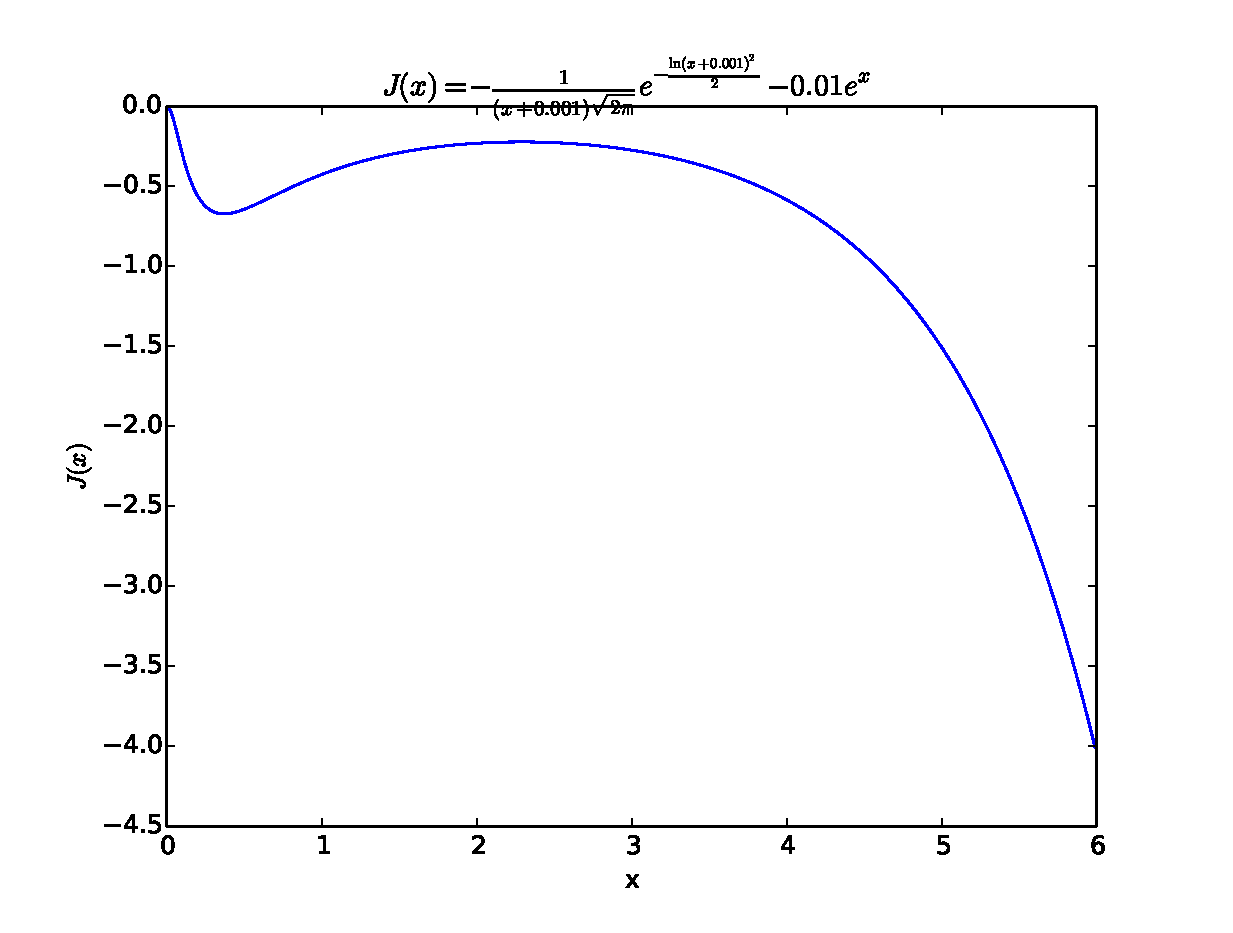
\includegraphics[width=1.0\linewidth]{exponential.eps}


\end{center}
   \caption{The plot of the cost function: $J(x) =-\frac{1}{(x+0.001) \sqrt{2 \pi}}e^{-\frac{\ln(x+0.001)^2}{2} }-0.01 e^x$. }
\label{fig:exp_cost_sphe}
\end{figure}





\begin{figure}[H]
\begin{center}
%\fbox{\rule{0pt}{2in} \rule{.9\linewidth}{0pt}}
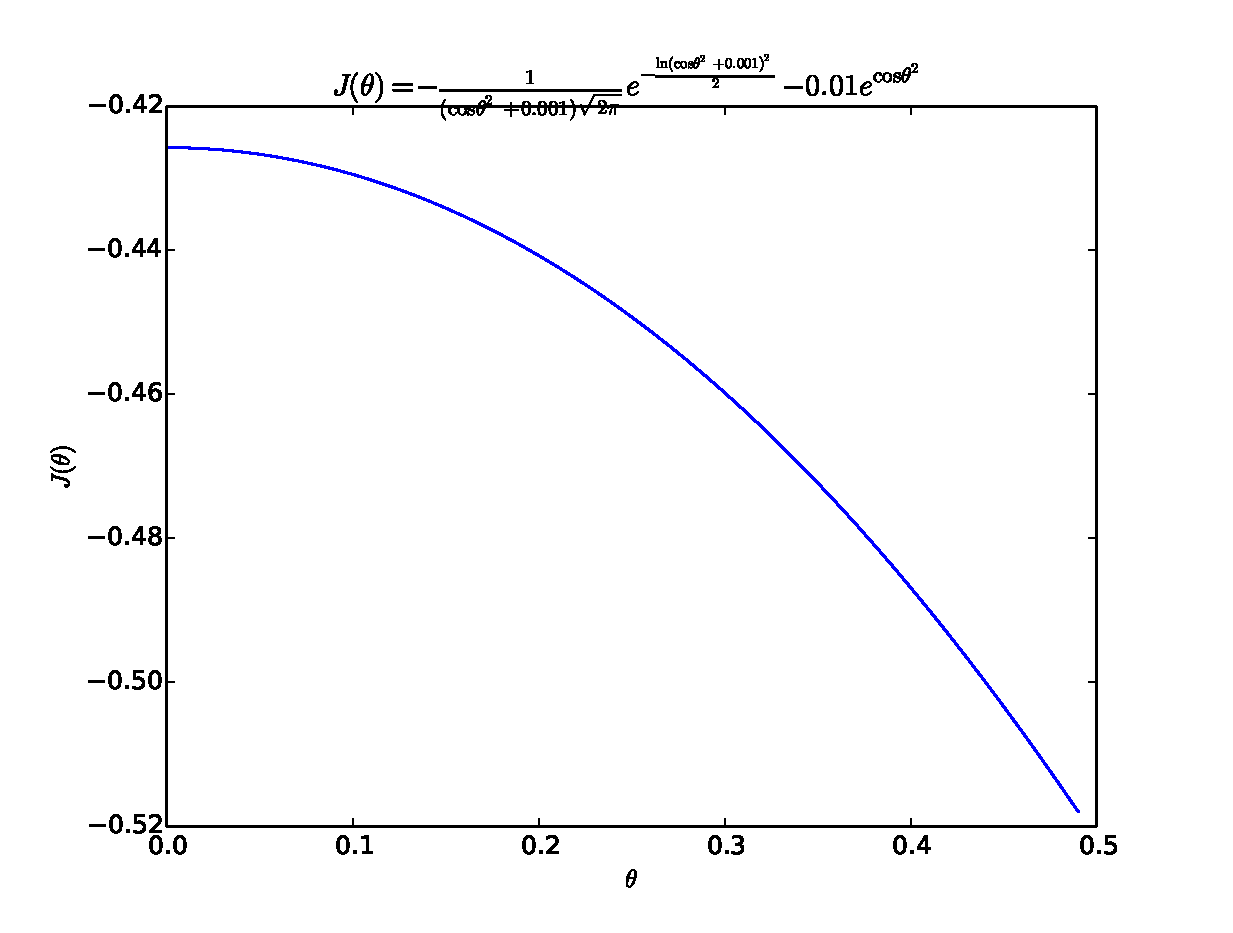
\includegraphics[width=1.0\linewidth]{exponential_sphe.eps}


\end{center}
   \caption{The plot of the cost function: $J(\theta)=-\frac{1}{(\cos \theta ^2+0.001) \sqrt{2 \pi}}e^{-\frac{\ln(\cos \theta ^2+0.001)^2}{2} }-0.01 e^{\cos \theta ^2}$. }
\label{fig:exp_cost_sphe}
\end{figure}





\subsubsection{Penalty method }
 By using the equation \ref{eq:pena_a}, equation \ref{eq:pena_b} and equation \ref{eq:pena_c}, for this specified question, we can get:\\
\begin{equation} \label{eq:pena_exp_a}
x_{n+1}=x_n-\epsilon _n \nabla J{\alpha_ n}(x_n)^T
\end{equation}
\begin{equation}\label{eq:pena_exp_b}
\alpha_{n+1}=\alpha_n+\delta _n \mathbbm{1} _{\{n\in {T_i}\}}
\end{equation}

\begin{equation}\label{eq:pena_exp_c}
\nabla _x J(x) =  -\frac{1+\ln(x+0.001)}{(x+0.001)^2 \sqrt{2 \pi}}e^{-\frac{\ln(x+0.001)^2}{2} }  -0.01 e^x
\end{equation}

\begin{equation}\label{eq:pena_exp_d}
\nabla J{\alpha_ n}(x_n) =\nabla _x J(x_n)+\alpha_n x_n( \mathbbm{1}_{\{x_n<0\}}+ x_n \mathbbm{1}_{\{x_n>1\}})
\end{equation}

By using the equation \ref{eq:pena_exp_a} , equation \ref{eq:pena_exp_b},  equation \ref{eq:pena_exp_c}  and equation \ref{eq:pena_exp_d}, we can estimate the optimal value of $x$ and the estimation process is shown in figure \ref{fig:poly_result}\\

\begin{figure}[H]
\begin{center}
%\fbox{\rule{0pt}{2in} \rule{.9\linewidth}{0pt}}
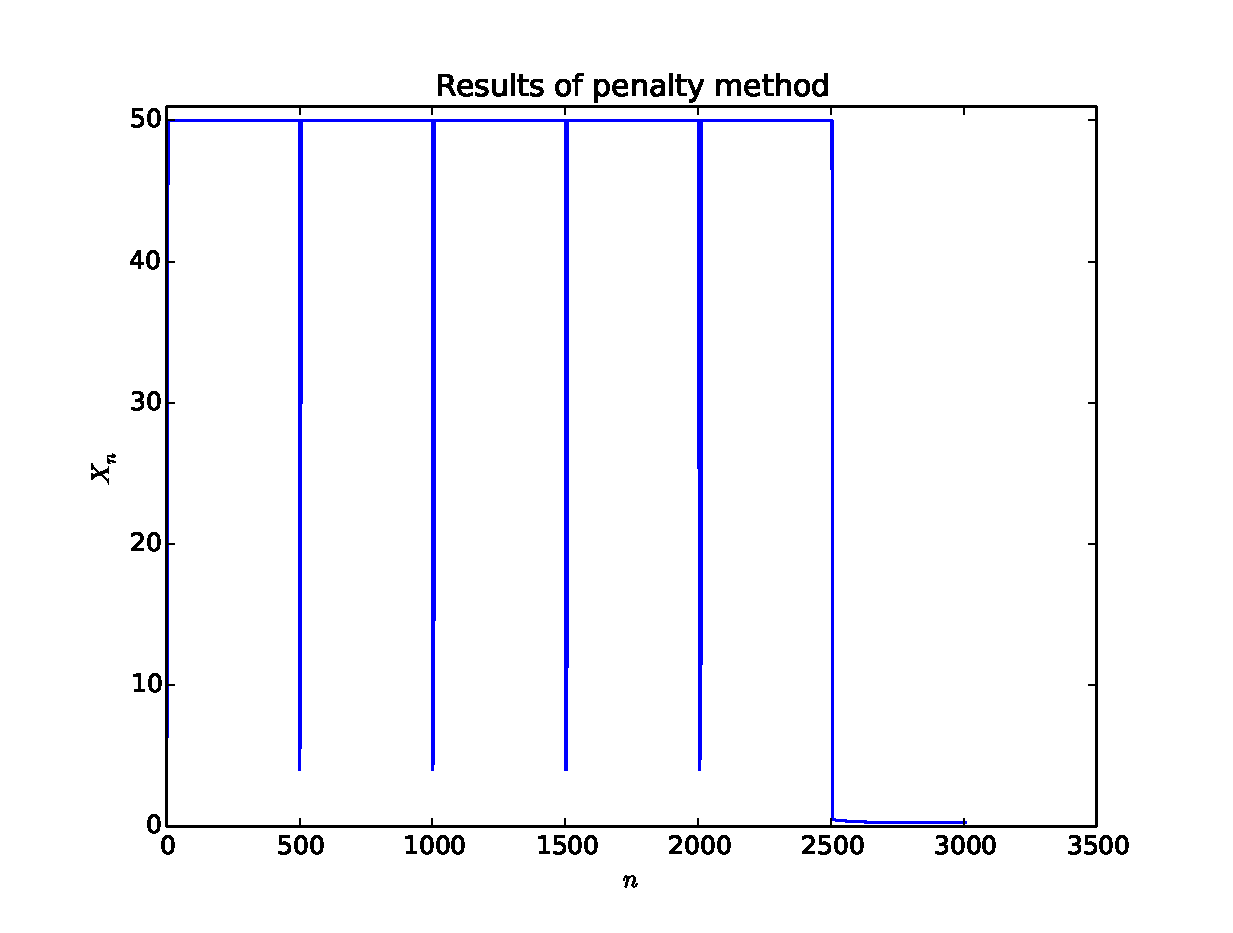
\includegraphics[width=1.0\linewidth]{polynomial_est.eps}


\end{center}
   \caption{The estimation process of the optimal $x$ when the penalty method is used.Here the initial value of $x$ is set to 4. The total iteration for $T_i$ is 500. The $\alpha_1 = 1$ and $\alpha _{n+1} = \alpha _n + \delta_n,$ where $\delta _ n=e^n$ The value of $x_n$ is upper bounded by the value of 50 as if it is not bounded, the value of $x_n$ will become too large to be handled by the computer. }
\label{fig:poly_result}
\end{figure}


\subsubsection{the spherical coordinated parameterization method }

\begin{equation} \label{eq:sphe_poly_a}
\theta_{n+1}=\theta_n-\epsilon _n \nabla J{\theta_ n}
\end{equation}
\begin{equation}\label{eq:sphe_poly_b}
\nabla _{\theta} J(\theta_n) = (\frac{1+\ln( \cos \theta ^2+0.001)}{( \cos \theta ^2+0.001)^2 \sqrt{2 \pi}}e^{-\frac{\ln( \cos \theta ^2+0.001)^2}{2} }  +0.01 e^ {\cos \theta ^2})(2 \cos \theta \sin \theta)
\end{equation}

When the spherical coordinated parameterization is used, the constrained optimization problem can be changed into a unconstrained problem. We can use the formula shown in equation \ref{eq:sphe_poly_a} and equation \ref{eq:sphe_poly_b} to estimate the optimal result. As we don't know whether the cost function is convex, we may get multiple local minimum. In order to get a global minimum, several experiments are done to get more than one estimation and the best one will be selected as the global optimization. In this experiment, 5 experiments are done. The estimation process is  shown in figure \ref{fig:polynomial_est_res_sphe}.\\



\begin{figure}[H]
\begin{center}
%\fbox{\rule{0pt}{2in} \rule{.9\linewidth}{0pt}}
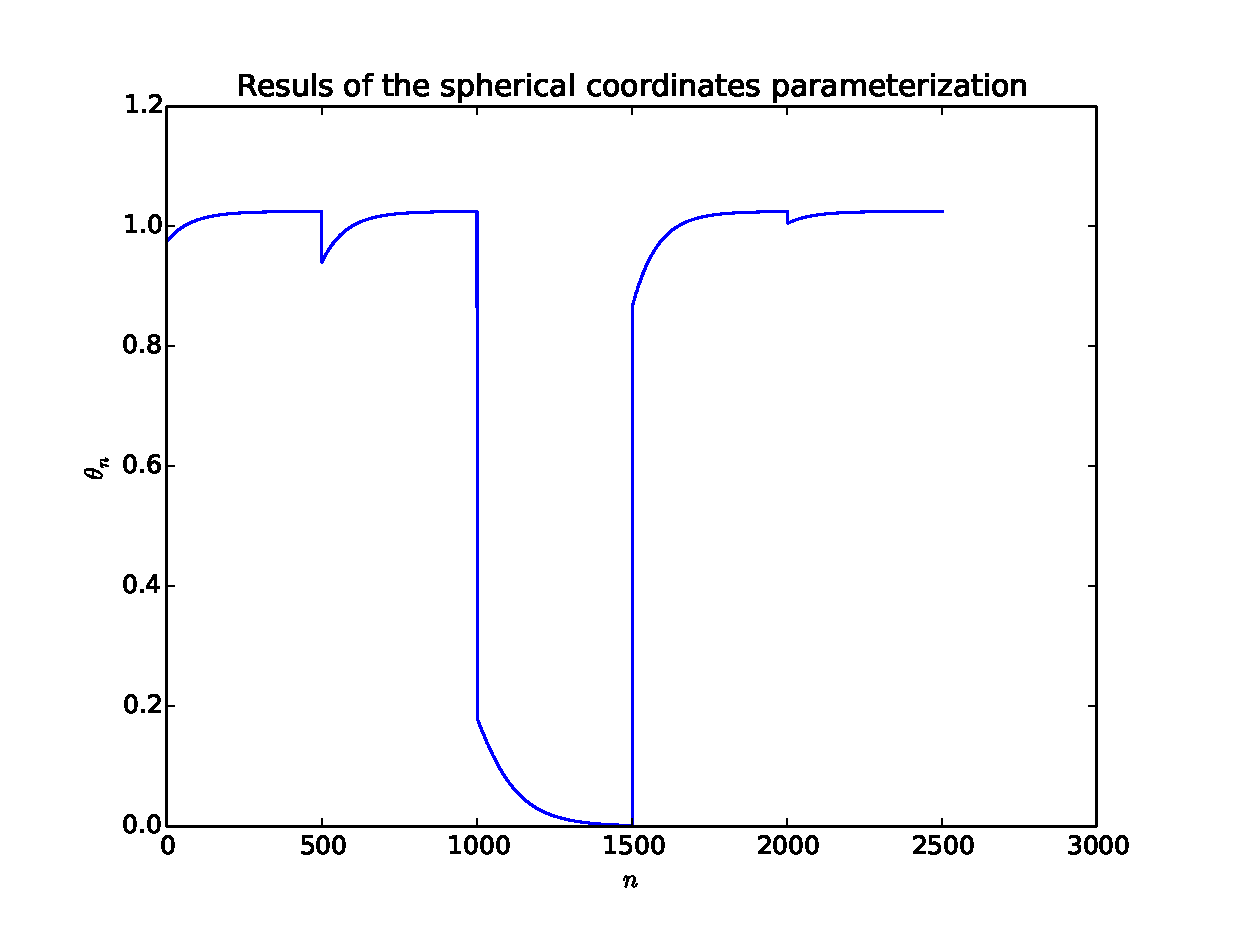
\includegraphics[width=1.0\linewidth]{polynomial_est_sphe.eps}


\end{center}
   \caption{The estimation process of the optimal $\theta$ when the spherical coordinated parameterization is used. In order to make sure the global optimal value is collected, 5 times experiments with random initialized value of $\theta$ is done and the global minimum value is collected from those 5 experiments.}
\label{fig:polynomial_est_res_sphe}
\end{figure}
\subsubsection{Optimization results comparison}

%owners-MacBook-Pro:project jimmy$ python polynomial.py 
%res 0.269693554986 0.269700164958
%--- 0.00234007835388 seconds ---
%owners-MacBook-Pro:project jimmy$ python polynomial_sphe.py 
%res 0.26962814355
%--- 0.0121109485626 seconds ---

\begin{table*}[!ht]
\begin{center}
\begin{tabular}{|c|c|c|c|}
\hline
Optimal $x$& method & estimated $x$&execution time(ms)\\
\hline
0.2696& penalty method&0.2697&2.34\\
\hline
0.2696&  \makecell{ the spherical coordinates \\parameterization}&0.2696&12.11\\

\hline
\end{tabular}
\end{center}
\caption{The results of the penalty method and spherical coordinate parameterization.}
\label{tab:poly}
\end{table*}


The comparison of the penalty and the spherical coordinates parameterization method is shown in table \ref{tab:poly}. We can get the similar conclusion as the cost function is linear. \\


\bibliography{jimmy_shen}
\bibliographystyle{ieeetr}
  
 \end{document}
